\documentclass[conference]{IEEEtran}
\usepackage{listings}
\usepackage[linesnumbered]{algorithm2e}
\usepackage[utf8]{inputenc}
\usepackage{multirow}
\usepackage{color}
\usepackage{pgfplots}

\usepackage{titlesec}

\newcommand{\comment}[2]{{\color{red}{#1: #2}}\\}

\usepackage[font=small,skip=2pt]{caption}
\setlength{\belowcaptionskip}{0.1cm}
\setlength{\textfloatsep}{0.1cm}

\usepackage{amssymb,amsmath}
\usepackage{ifxetex,ifluatex}
\usepackage{fixltx2e} % provides \textsubscript

\ifnum 0\ifxetex 1\fi\ifluatex 1\fi=0 % if pdftex
  \usepackage[T1]{fontenc}
  \usepackage[utf8]{inputenc}
\else % if luatex or xelatex
  \ifxetex
    \usepackage{mathspec}
    \usepackage{xltxtra,xunicode}
  \else
    \usepackage{fontspec}
  \fi
  \defaultfontfeatures{Mapping=tex-text,Scale=MatchLowercase}
  \newcommand{\euro}{€}


\fi
% use upquote if available, for straight quotes in verbatim environments
\IfFileExists{upquote.sty}{\usepackage{upquote}}{}
% use microtype if available
\IfFileExists{microtype.sty}{%
\usepackage{microtype}
\UseMicrotypeSet[protrusion]{basicmath} % disable protrusion for tt fonts
}{}


\ifxetex
  \usepackage[setpagesize=false, % page size defined by xetex
              unicode=false, % unicode breaks when used with xetex
              xetex]{hyperref}
\else
  \usepackage[unicode=true]{hyperref}
\fi
\hypersetup{breaklinks=true,
            bookmarks=true,
            pdfauthor={},
            pdftitle={BIANCA: Preventing Bug Insertion at Commit-Time Using Dependency Analysis and Clone Detection},
            colorlinks=true,
            citecolor=blue,
            urlcolor=blue,
            linkcolor=magenta,
            pdfborder={0 0 0}}
\urlstyle{same}  % don't use monospace font for urls




\usepackage{color}
\usepackage{fancyvrb}
\newcommand{\VerbBar}{|}
\newcommand{\VERB}{\Verb[commandchars=\\\{\}]}
\DefineVerbatimEnvironment{Highlighting}{Verbatim}{commandchars=\\\{\}}
% Add ',fontsize=\small' for more characters per line
\newenvironment{Shaded}{}{}
\newcommand{\KeywordTok}[1]{\textcolor[rgb]{0.00,0.44,0.13}{\textbf{{#1}}}}
\newcommand{\DataTypeTok}[1]{\textcolor[rgb]{0.56,0.13,0.00}{{#1}}}
\newcommand{\DecValTok}[1]{\textcolor[rgb]{0.25,0.63,0.44}{{#1}}}
\newcommand{\BaseNTok}[1]{\textcolor[rgb]{0.25,0.63,0.44}{{#1}}}
\newcommand{\FloatTok}[1]{\textcolor[rgb]{0.25,0.63,0.44}{{#1}}}
\newcommand{\CharTok}[1]{\textcolor[rgb]{0.25,0.44,0.63}{{#1}}}
\newcommand{\StringTok}[1]{\textcolor[rgb]{0.25,0.44,0.63}{{#1}}}
\newcommand{\CommentTok}[1]{\textcolor[rgb]{0.38,0.63,0.69}{\textit{{#1}}}}
\newcommand{\OtherTok}[1]{\textcolor[rgb]{0.00,0.44,0.13}{{#1}}}
\newcommand{\AlertTok}[1]{\textcolor[rgb]{1.00,0.00,0.00}{\textbf{{#1}}}}
\newcommand{\FunctionTok}[1]{\textcolor[rgb]{0.02,0.16,0.49}{{#1}}}
\newcommand{\RegionMarkerTok}[1]{{#1}}
\newcommand{\ErrorTok}[1]{\textcolor[rgb]{1.00,0.00,0.00}{\textbf{{#1}}}}
\newcommand{\NormalTok}[1]{{#1}}



\usepackage{titlesec}

\titlespacing\section{0pt}{0pt plus 0pt minus 0pt}{0pt plus 0pt minus 0pt}
\titlespacing\subsection{0pt}{0pt plus 0pt minus 0pt}{0pt plus 0pt minus 0pt}
\titlespacing\subsubsection{0pt}{0pt plus 0pt minus 0pt}{0pt plus 0pt minus 0pt}



\setlength{\parindent}{0pt}
\setlength{\parskip}{6pt plus 2pt minus 1pt}
\setlength{\emergencystretch}{3em}  % prevent overfull lines
\providecommand{\tightlist}{%
  \setlength{\itemsep}{0pt}\setlength{\parskip}{0pt}}
\setcounter{secnumdepth}{5}


\title{\vspace{-1cm}BIANCA: Preventing Bug Insertion at Commit-Time Using Dependency
Analysis and Clone Detection}

\author{  \IEEEauthorblockN{Mathieu Nayrolles, Abdelwahab Hamou-Lhadj} \IEEEauthorblockA{ SBA Lab, ECE Dept, Concordia University \\ Montréal, QC, Canada \\ {\footnotesize\texttt{\{mathieu.nayrolles, wahab.hamou-lhadj\}@concordia.ca}} \\ \\\vspace{-1.5cm}}  \and  \IEEEauthorblockN{Emad Shihab} \IEEEauthorblockA{ DAS Lab, CSE Dept, Concordia University \\ Montréal, QC, Canada \\ {\footnotesize\texttt{eshihab@cse.concordia.ca}} \\ \vspace{-1.5cm}} }

\begin{document}
\maketitle
\begin{abstract}
Preventing the introduction of software defects at commit-time is a
growing line of research in the software maintenance community. Existing
approaches leverage code and process metrics to build statistical models
that can effectively prevent defect insertion and propose fixes in a
software project. Metrics, however, may vary from one project to
another, hindering the reuse of these models. Moreover, these techniques
operate within single projects only despite the fact that many projects
share dependencies and are, therefore, vulnerable to similar faults. In
this paper, we propose a novel approach, called BIANCA, that relies on
clone detection and dependency analysis to detect \emph{risky} commits
within and across related projects. When applied to 42 projects, BIANCA
achieves an average precision, recall and F-measure of 90.75\%, 37.15\%
and 52.72\%, respectively. We also found that only 8.6\% of the risky
commits detected by BIANCA match other commits from the same project,
suggesting that relationships across projects need to be considered for
effective prevention of risky commits. In addition, BIANCA is able to
propose qualitative fixes to transform \emph{risky} commits into
\emph{non-risky} ones in 78.67\% of the cases.
\end{abstract}

\begin{IEEEkeywords}
    Bug Prediction;
    Risky Software Commits;
    Clone Detection;
    Software Maintenance\end{IEEEkeywords}



\section{Introduction}\label{introduction}

Research in software maintenance continues to evolve to include areas
like mining bug repositories, bug analytic, and bug prevention and
reproduction. The ultimate goal is to develop techniques and tools to
help software developers detect, correct, and prevent bugs in an
effective and efficient manner.

One particular (and growing) line of research focuses on the problem of
preventing the introduction of bugs by detecting risky commits
(preferably before the commits reach the central repository). Recent
approaches (e.g., {[}1{]}, {[}2{]}) rely on training models based on
code and process metrics (e.g., code complexity, experience of the
developers, etc.) that are used to classify new commits as risky or not.
Metrics, however, may vary from one project to another, hindering the
reuse of these models. Consequently, these techniques tend to operate
within single projects only, despite the fact many large projects share
dependencies such as the reuse of common libraries. This makes them
potentially vulnerable to similar faults. A solution to a bug provided
by the developers of one project may help fix a bug that occur in
another (and dependant) project. Moreover, as noted by Lewis \emph{et
al.} {[}3{]} and Johnson \emph{et al.} {[}4{]}, techniques based solely
on metrics are perceived by developers as black box solutions because
they do not provide any insights on the causes of the risky commits or
ways for improving them. As a result, developers are less likely to
trust the output of these tools.

In this paper, we propose a novel bug prevention approach at
commit-time, called BIANCA (Bug Insertion ANticipation by Clone Analysis
at commit time). BIANCA does not use metrics to assess whether or not an
incoming commit is risky. Instead, it relies on code clone detection
techniques by extracting code blocks from incoming commits and comparing
them to those of known defect-introducing commits.

One particular aspect of BIANCA is its ability to detect risky commits
not only by comparing them to commits of a single project but also to
those belonging to other projects that share common dependencies. This
is important because complex software systems are not designed in a
monolithic way. They have dependencies that make them vulnerable to
similar faults. For example, Apache BatchEE {[}5{]} and GraphWalker
{[}6{]} both depend on JUNG (Java Universal Network/Graph Framework)
{[}7{]}. BatchEE provides an implementation of the jsr-352 (Batch
Applications for the Java Platform) specification {[}8{]} while
GraphWalker is an open source model-based testing tool for test
automation. These two systems are designed for different purposes.
BatchEE is used to do batch processing in Java, whereas GraphWalker is
used to design unit tests using a graph representation of code.
Nevertheless, because both Apache BatchEE and GraphWalker rely on JUNG,
the developers of these projects made similar mistakes when building
upon JUNG. The issue reports Apache BatchEE \#69 and GraphWalker \#44
indicate that the developers of these projects made similar mistakes
when using the graph visualization component of JUNG. To detect commits
across related projects, BIANCA resorts to project dependency analysis.

Another advantage of BIANCA is that it uses commits that are used to fix
previous defect-introducing commits to provide guidance to the
developers on how to improve risky commits. This way, BIANCA goes one
step further than existing techniques by providing developers with a
potential fix for their risky commits.

We validated the performance of BIANCA on 42 open source projects,
obtained from Github. The examined projects vary in size, domain and
popularity. Our findings indicate that BIANCA is able to flag risky
commits with an average precision, recall and F-measure of 90.75\%,
37.15\% and 52.72\%, respectively. Moreover, we found that only 8.6\% of
the risky commits detected by BIANCA match other commits from the same
project. This finding stresses the fact that relationships across
projects should be taken into consideration for effective prevention of
risky commits.

The remaining parts of this paper are organized as follows. In Section
\ref{sec:relwork}, we present related work. Sections \ref{sec:bianca},
\ref{sec:exp} and \ref{sec:result} are dedicated to the BIANCA approach,
the case study setup, and the case study results. Then, Sections
\ref{sec:threats} and \ref{sec:conclusion} present the threats to
validity and a conclusion accompanied with future work.

\section{Related Work}\label{sec:relwork}

The work most related to ours comes from two main areas, work that aims
to predict future defects in files, modules and changes and work that
aims to propose or generate patches for buggy software.

\subsection{File, Module and Risky Change
Prediction}\label{file-module-and-risky-change-prediction}

The majority of previous file/module-level prediction work used code or
process metrics. Approaches using code metrics only use information from
the code itself and do not use any historical data. Chidamber and
Kemerer published the well-known CK metrics suite {[}9{]} for object
oriented designs and inspired Moha \emph{et al.} to publish similar
metrics for service-oriented programs {[}10{]}. Another famous metric
suite for assessing the quality of a given software design is Briand's
coupling metrics {[}11{]}.

The CK and Briand's metrics suites have been used, for example, by
Basili \emph{et al.} {[}12{]}, El Emam \emph{et al.} {[}13{]},
Subramanyam \emph{et al.} {[}14{]} and Gyimothy \emph{et al.} {[}15{]}
for object-oriented designs. Service oriented designs have been far less
studied than object oriented design as they are relatively new, but,
Nayrolles \emph{et al.} {[}16{]}, {[}17{]}, Demange \emph{et al.}
{[}18{]} and Palma \emph{et al.} {[}19{]} used Moha \emph{et al.} metric
suites to detect software defects. All these approaches, proved software
metrics to be useful at detecting software fault for object oriented and
service oriented designs, respectively. More recently, Nagappan \emph{et
al.} {[}20{]}, {[}21{]} and Zimmerman \emph{et al.} {[}22{]}, {[}23{]}
further refined metrics-based detection by using statical analysis and
call-graph analysis.

Other approaches use historical development data, often referred to as
process metrics. Naggapan and Ball {[}24{]} studied the feasibility of
using relative churn metrics to prediction buggy modules in the Windows
Server 2003. Other work by Hassan \emph{et al} and Ostrand \emph{et al}
used past changes and defects to predict buggy locations (e.g.,
{[}25{]}, {[}26{]}). Hassan and Holt proposed an approach that
highlights the top ten most susceptible locations to have a bug using
heuristics based on file-level metrics {[}25{]}. They find that
locations that have been recently modified and fixed locations are the
most defect-prone. Similarly, Ostrand \emph{et al.} {[}26{]} predict
future crash location by combining the data from changed and past defect
locations. They validate their approach on industrial systems at AT\&T.
They showed that data from prior changes and defects can effectively
defect-prone locations for open-source and industrial systems. Kim
\emph{et al.} {[}27{]} proposed the bug cache approach, which is an
improved technique over Hassan and Holt's approach {[}25{]}. Rahman and
Devanbu found that, in general, process-based metrics perform as good as
or better than code-based metrics {[}28{]}.

Other work focused on the prediction of risky changes. Kim et al.
proposed the change classification problem, which predicts whether a
change is buggy or clean {[}29{]}. Hassan {[}30{]} used the entropy of
changes to predict risky changes. They find that the more complex a
change is, the more likely it is to introduce a defect. Kamei \emph{et
al.} performed a large-scale empirical study on change classification
{[}31{]}. They aforementioned studies find that size of a change and the
history of the files being changed (i.e., how buggy they were in the
past) are the best indicators of risky changes.

Our work shares a similar goal to the work on the prediction of risky
changes, however, BIANCA takes a different approach in that it leverages
dependencies of a project to determine risky changes.

\subsection{Automatic Patch
Generation}\label{automatic-patch-generation}

Since BIANCA not only flags risky changes, but also provides developers
with fixes that have been applied in the past, automatic patch
generation work is also related. Pan \emph{et al.} {[}32{]} identified
27 bug fixing patterns that can be applied to fix software bugs in Java
programs. They showed that between 45.7 - 63.6\% of the bugs can be
fixed with their patterns. Later, Kim \emph{et al.} {[}33{]} generated
patches from human-written patches and showed that their tool, PAR,
successfully generated patches for 27 of 119 bugs. Tao \emph{et al.}
{[}34{]} also showed that automatically generated patches can assist
developers in debugging tasks. Other work also focused on determining
how to best generate acceptable and high quality patches, e.g. {[}35{]},
{[}36{]}, and determine what bugs are best fit for automatic patch
generation {[}37{]}.

Our work differs from the work on automated patch generation in that we
do not generate patches, rather we use clone detection to determine the
similarity of a change to a previous risky change and suggest to the
developer the fixes of the prior risky changes.

\section{The BIANCA Approach}\label{sec:bianca}

Figures \ref{fig:bianca1}, \ref{fig:bianca3} and \ref{fig:bianca2} show
an overview of the BIANCA approach, which consists of two parallel
processes.

In the first process (Figures \ref{fig:bianca1} and \ref{fig:bianca3}),
BIANCA manages events happening on project tracking systems to extract
defect-introducing commits and commits that provided the fixes. For
simplicity, in the rest of this paper, we refer to commits that are used
to fix defects as \emph{fix-commits}. We use the term
\emph{defect-commit} to mean a commit that introduces a defect. In the
second phase, BIANCA analyses the developer's new commits before they
reach the central repository to detect potential risky commits (commits
that may introduce bugs).

\begin{figure*}
  \centering
    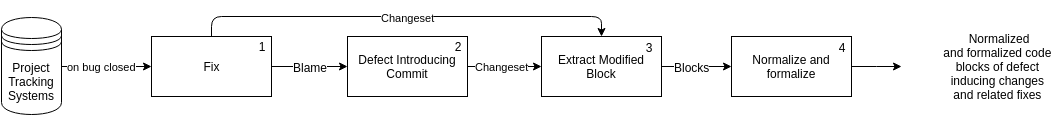
\includegraphics[width=\textwidth]{media/fix-approach.png}
    \caption{Managing events happening on project tracking systems to extract defect-introducing commits and commits that provided the fixes\label{fig:bianca1}}
\end{figure*}

\begin{figure*}
  \centering
    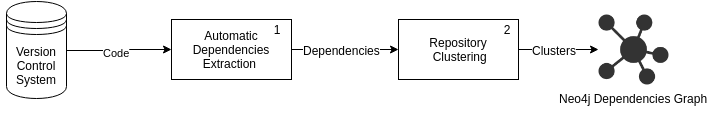
\includegraphics[width=0.8\textwidth]{media/cluster-approach}
    \caption{Clustering by dependency\label{fig:bianca3}}
\end{figure*}

\begin{figure*}
  \centering
    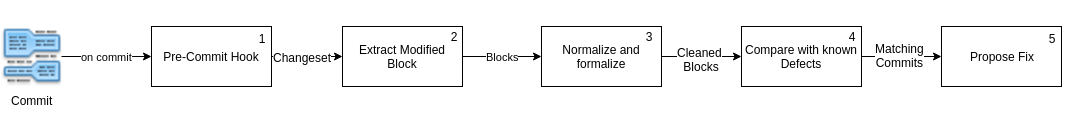
\includegraphics[width=\textwidth]{media/detect-approach}
    \caption{Classifying incoming commits and proposing fixes\label{fig:bianca2}}
\end{figure*}



The project tracking component of BIANCA listens to bug (or issue)
closing events of major open-source projects (currently, BIANCA is
tested with 42 large projects). These projects share many dependencies.
Projects can depend on each other or on common external tools and
libraries. We perform project dependency analysis to identify groups of
highly-coupled projects.

In the second process (Figure \ref{fig:bianca2}), BIANCA identifies
risky commits within each group so as to increase the chances of finding
risky commits caused by project dependencies. For each project group, we
extract code blocks from defect-commits and fix-commits.\\The extracted
code blocks are saved in a database that is used to identify risky
commits before they reach the central repository. For each match between
a risky commit and a defect-commit, we pull out from the database the
corresponding \emph{fix-commit} and present it to the developer as a
potential way to improve the commit content. These phases are discussed
in more detail in the upcoming subsections.

\subsection{Clustering Project Repositories}\label{sec:clustering}

We cluster projects according to their dependencies. The rationale is
that projects that share dependencies are most likely to contain defects
caused by misuse of these dependencies. In this step, the project
dependencies are analysed and saved into a single no-SQL graph database
as shown in Figure \ref{fig:bianca3}. Graph databases use graph
structures as a way to store and query information. In our case, a node
corresponds to a project that is connected to other projects on which it
depends. Project dependencies can be automatically retrieved if projects
use a dependency manager such as Maven.

Figure \ref{fig:network-sample} shows a simplified view of a dependency
graph for a project named \texttt{com.badlogicgames.gdx}. As we can see,
\texttt{badlogicgames.gdx} depends on projects owned by the same
organization (i.e., badlogicgames) and other organizations such as
Google, Apple, and Github.

\begin{figure*}
  \centering
    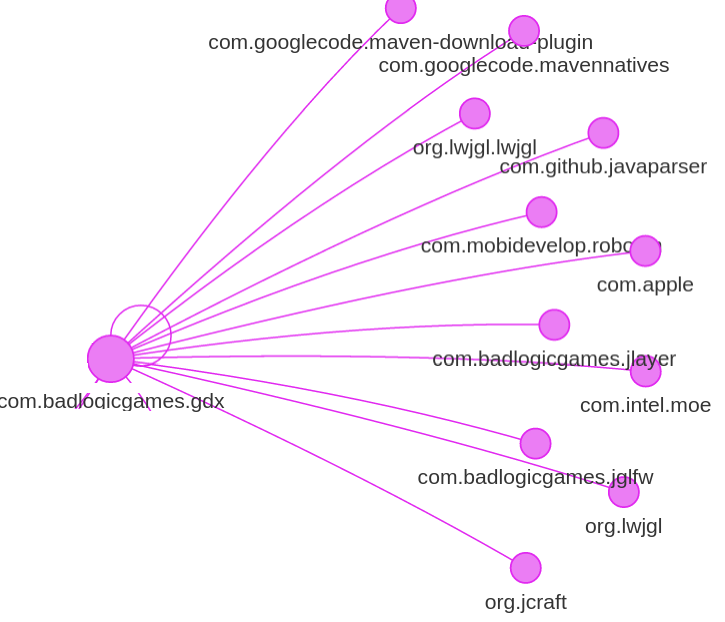
\includegraphics[width=0.60\textwidth]{media/network-sample.png}
    \caption{Simplified Dependency Graph for \texttt{com.badlogicgames.gdx}\label{fig:network-sample}}
\end{figure*}

Once the project dependency graph is extracted, we use a clustering
algorithm to partition the graph. To this end, we choose the
Girvan--Newman algorithm {[}38{]}, {[}39{]}, used to detect communities
by progressively removing edges from the original network. The connected
components of the remaining network form distinct communities. Instead
of trying to construct a measure that identifies the edges that are the
most central to communities, the Girvan--Newman algorithm focuses on
edges that are most likely ``between'' communities. This algorithm is
very effective at discovering community structure in both
computer-generated and real-world network data {[}39{]}. Other
clustering algorithms can also be used.

\subsection{Building a Database of Code Blocks of Defect-Commits and
Fix-Commits}\label{sec:offline}

To build our database of code blocks that are related to defect-commits
and fix-commits, we first need to identify the respective commits. Then,
we extract the relevant blocks of code from the commits.

\textbf{Extracting Commits:} BIANCA listens to bug (or issue) closing
events happening on the project tracking system. Every time an issue is
closed, BIANCA retrieves the commit that was used to fix the issue (the
fix-commit) as well as the one that introduced the defect (the
defect-commit). Retrieving fix-commits, however, is known to be a
challenging task {[}40{]}. This is because the link between the project
tracking system and the code version control system is not always
explicit. In an ideal situation, developers would add a reference to the
issue they work on inside the description of the commit. But this good
practice is not always followed. To make the link between fix-commits
and their related issues, we turn to a modified version of the back-end
of commit-guru {[}41{]}. Commit-guru is a tool, developed by Rosen
\emph{et al.} {[}41{]} to detect \emph{risky commits}. In order to
identify risky commits, Commit-guru builds a statistical model using
change metrics (i.e., amount of lines added, amount of lines deleted,
amount of files modified, etc.) from past commits known to have
introduced defects in the past.

Commit-guru's back-end has three major components: ingestion, analysis,
and prediction. We reuse the ingestion part of the analysis components
for BIANCA. The ingestion component is responsible for ingesting (i.e.,
downloading) a given repository. Once the repository is entirely
downloaded on a local server, each commit history is analysed. Commits
are classified using the list of keywords proposed by Hindle \emph{et
al.} {[}42{]}. Commit-guru implements the SZZ algorithm {[}43{]} to
detect risky changes, where it performs the SCM blame/annotate function
on all the modified lines of code for their corresponding files on the
fix-commit's parents. This returns the commits that previously modified
these lines of code and are flagged as the bug introducing commits
(i.e., the defect-commits). Priori work showed that Commit-guru is
effective in identifying defect-commits and their corresponding fixing
commits {[}44{]} and to date, the SZZ algorithm, which Commit-guru uses,
is considered to be the state-of-the-art in detecting risky commits.
Note that we could use a simpler and more established tool such as
Relink {[}40{]} to link the commits to their issues and re-implement the
classification proposed by Hindle \emph{et al.} {[}42{]} on top of it.
However, commit-guru has the advantage of being open-source, making it
possible to modify it to fit our needs and fine-tune its performance.

\textbf{Extracting Code Blocks:} To extract code blocks from fix-commits
and defect-commits, we rely on TXL {[}45{]}, which is a first-order
functional programming over linear term rewriting, developed by Cordy et
al. {[}45{]}. For TXL to work, one has to write a grammar describing the
syntax of the source language and the transformations needed. TXL has
three main phases: \emph{parse}, \emph{transform}, \emph{unparse}. In
the parse phase, the grammar controls not only the input but also the
output forms. The following code sample---extracted from the official
documentation---shows a grammar matching an \emph{if-then-else}
statement in C with some special keywords: {[}IN{]} (indent), {[}EX{]}
(exdent) and {[}NL{]} (newline) that will be used in the output form.

\begin{Shaded}
\begin{Highlighting}[]
\KeywordTok{define} \NormalTok{if_statement}
  \KeywordTok{if} \KeywordTok{(} \NormalTok{[}\KeywordTok{expr}\NormalTok{] }\KeywordTok{)} \NormalTok{[}\KeywordTok{IN}\NormalTok{][NL]}
\NormalTok{[}\KeywordTok{statement}\NormalTok{] [EX]}
\NormalTok{[}\KeywordTok{opt} \NormalTok{else_statement]}
\KeywordTok{end} \NormalTok{define}

\KeywordTok{define} \NormalTok{else_statement}
  \KeywordTok{else} \NormalTok{[}\KeywordTok{IN}\NormalTok{][NL]}
\NormalTok{[}\KeywordTok{statement}\NormalTok{] [EX]}
\KeywordTok{end} \NormalTok{define}
\end{Highlighting}
\end{Shaded}

Then, the \emph{transform} phase applies transformation rules that can,
for example, normalize or abstract the source code. Finally, the third
phase of TXL, called \emph{unparse}, unparses the transformed parsed
input to output it. Also, TXL supports what its creators call
\emph{Agile Parsing} {[}46{]}, which allow developers to redefine the
rules of the grammar and, therefore, apply different rules than the
original ones. BIANCA takes advantage of that by redefining the blocks
that should be extracted for the purpose of code comparison, leaving out
the blocks that are out of scope. More precisely, before each commit, we
only extract the blocks belonging to the modified parts of the source
code. Hence, we only process, in an incremental manner, the latest
modification of the source code instead of the source code as a whole.


We have selected TXL for several reasons. First, TXL is easy to install
and to integrate with the normal work flow of a developer. Second, it
was relatively easy to create a grammar that accepts commits as input.
This is because TXL supports C, Java, Csharp, Python and WSDL grammars,
with the ability to customize them to accept changesets (chunks of the
modified source code that include the added, modified, and deleted
lines) instead of the whole code.


Algorithm \ref{alg:extract} presents an overview of the \emph{extract}
and \emph{save} blocks operations of BIANCA. This algorithm receives as
argument, the changesets and the blocks that have been previously
extracted. Then, Lines 1 to 5 show the $for$ loop that iterates over the
changesets. For each changeset (Line 2), we extract the blocks by
calling the $~extract\_blocks(Changeset~cs)$ function. In this function,
we expand our changeset to the left and to the right in order to have a
complete block.


\begin{algorithm}
 \KwData{$Changeset[]$ changesets\;
 $Block[]$ prior\_blocks\;
 }
 \KwResult{Up to date blocks of the systems}
 \For{$i \leftarrow 0$ \KwTo$size\_of~changesets$}{
    Block[] blocks $\leftarrow$ $extract\_blocks(changesets)$\;
    \For{$j \leftarrow 0$ \KwTo$size\_of~blocks$}{
       write $blocks[j]$\;
    }
 }

 \SetKwProg{myproc}{Function}{ $~extract\_blocks(Changeset~cs)$}{}
   \myproc{{}}{

   \uIf{$cs~is~unbalanced~right$}{$cs \leftarrow expand\_left(cs)$\;}

   \ElseIf{$cs~is~unbalanced~left$}{$cs \leftarrow expand\_right(cs)$\;}

   \nl\KwRet$txl\_extract\_blocks(cs)$\;
   }


 \caption{Overview of the Extract Blocks Operation\label{alg:extract}}
\end{algorithm}

As depicted below, changesets contain only the modified chunk of code
and not necessarily complete blocks.

\begin{Shaded}
\begin{Highlighting}[]
\DataTypeTok{@@ -315,36 +315,6 @@}
\NormalTok{int initprocesstree_sysdep}
\NormalTok{(ProcessTree_T **reference) \{}
    \NormalTok{mach_port_deallocate(mytask,}
      \NormalTok{task);}
\NormalTok{\}}
\NormalTok{\}}
\StringTok{- if (task_for_pid(mytask, pt[i].pid,}
\StringTok{-  &task) == KERN_SUCCESS) \{}
\StringTok{-   mach_msg_type_number_t   count;}
\StringTok{-   task_basic_info_data_t   taskinfo;}
\end{Highlighting}
\end{Shaded}

Therefore, we need to expand the changeset to the left (or right) to
have syntactically correct blocks. We do so by checking the block's
beginning and ending with a parentheses algorithms {[}47{]}. Then, we
send these expanded changesets to TXL for block extraction and
formalization.

One important note about this database is that the process can be
cold-started. A tool supporting BIANCA does not need to \emph{wait} for
a project to have issues and fixes to be in effect. It can leverage the
defect-commits and fix-commits of projects in the same cluster that
already have a history. Therefore, BIANCA is applicable at the beginning
of every project. The only requirement is to use a dependency manager.

\subsection{Analysing New Commits Using Pre-Commit
Hooks}\label{sec:online}

Each time a developer makes a commit, BIANCA intercepts it using a
pre-commit hook, extracts the corresponding code block (in a similar way
as in the previous phase), and compares it to the code blocks of
historical defect-commits. If there is a match then the new commit is
deemed to be risky. A threshold $\alpha$ is used to assess the extent
beyond which two commits are considered similar. The setting of $\alpha$
is discussed in the case study section.

Pre-commit hooks are custom scripts set to fire off when certain
important actions of the versionning process occur. There are two groups
of hooks: client-side and server-side. Client-side hooks are triggered
by operations such as committing and merging, whereas server-side hooks
run on network operations such as receiving pushed commits. These hooks
can be used for all sorts of reasons such as checking compliance with
coding rules or automatic run of unit test suites. The pre-commit hook
runs before the developer specifies a commit message. It is used to
inspect the modifications that are about to be committed. BIANCA is
based on a set of bash and python scripts, and the entry point of these
scripts lies in a pre-commit hook. These scripts intercept the commit
and extract the corresponding code blocks.

To compare the extracted blocks to the ones in the database, we resort
to clone detection techniques, more specifically, text-based clone
detection techniques. This is because lexical and syntactic analysis
approaches (alternatives to text-based comparisons) would require a
complete program to work, i.e., a program that compiles. In the
relatively wide-range of tools and techniques that exist to detect
clones by considering code as text {[}48--53{]}, we selected NICAD as
the main text-based method for comparing code blocks {[}54{]} for
several reasons. First, NICAD is built on top of TXL, which we also used
in the previous phase. Second, NICAD can detect Types 1, 2 and 3
software clones {[}55{]}. Type 1 clones are copy-pasted blocks of code
that only differ from each other in terms of non-code artefacts such as
indentation, whitespaces, comments and so on. Type 2 clones are blocks
of code that are syntactically identical except literals, identifiers,
and types that can be modified. Also, Type 2 clones share the
particularities of Type 1 about indentation, whitespaces, and comments.
Type 3 clones are similar to Type 2 clones in terms of modification of
literals, identifiers, types, indentation, whitespaces, and comments but
also contain added or deleted code statements. BIANCA detects Type 3
clones since they can contain added or deleted code statements, which
make them suitable for comparing commit code blocks.

NICAD works in three phases: \emph{Extraction}, \emph{Comparison} and
\emph{Reporting}. During the \emph{Extraction} phase all potential
clones are identified, pretty-printed, and extracted. We do not use the
\emph{Extraction} phase of NICAD as it has been built to work on
programs that are syntactically correct, which is not the case for
changesets. We replaced NICAD's \emph{Extraction} phase with our scripts
for building code blocks (described in the previous phase).

In the \emph{Comparison} phase, the extracted blocks are transformed,
clustered and compared to find potential clones. Using TXL sub-programs,
blocks go through a process called pretty-printing where they are
stripped of formatting and comments. When code fragments are cloned,
some comments, indentation or spacing are changed according to the new
context where the new code is used. This pretty-printing process ensures
that all code will have the same spacing and formatting, which renders
the comparison of code fragments easier. Furthermore, in the
pretty-printing process, statements can be broken down into several
lines. Table \ref{tab:pretty-printing} {[}56{]} shows how this can
improve the accuracy of clone detection with three \texttt{for}
statements, \texttt{for (i=0; i\textless{}10; i++)},
\texttt{for (i=1; i\textless{}10; i++)} and
\texttt{for (j=2; j\textless{}100; j++)}. The pretty-printing allows
NICAD to detect Segments 1 and 2 as a clone pair because only the
initialization of $i$ changed. This specific example would not have been
marked as a clone by other tools we tested such as Duploc {[}57{]}. In
addition to the pretty-printing, code can be normalized and filtered to
detect different classes of clones and match user preferences.

\begin{table}[]
\centering
\caption{Pretty-Printing Example}
\label{tab:pretty-printing}
\resizebox{0.5\textwidth}{!}{%
\begin{tabular}{l|l|l|l|l|l}
\hline
Segment 1          & Segment 2          & Segment 3           & S1 \& S2 & S1 \& S3 & S2 \& S3 \\ \hline \hline
for (              & for (              & for (               & 1        & 1        & 1        \\
i = 0;             & i = 1;             & j = 2;              & 0        & 0        & 0        \\
i \textgreater 10; & i \textgreater 10; & j \textgreater 100; & 1        & 0        & 0        \\ 
i++)               & i++)               & j++)                & 1        & 0        & 0        \\ \hline \hline
\multicolumn{3}{c|}{Total Matches}                            & 3        & 1        & 1        \\ \hline
\multicolumn{3}{c|}{Total Mismatches}                         & 1        & 3        & 3 \\ \hline

\end{tabular}
}
\end{table}


The extracted, pretty-printed, normalized and filtered blocks are marked
as potential clones using a Longest Common Subsequence (LCS) algorithm
{[}58{]}. Then, a percentage of unique statements can be computed and,
given the threshold $\alpha$, the blocks are marked as clones.

Another important aspect of the design of BIANCA is the ability to
provide guidance to developers on how to improve the risky commits. We
achieve this by extracting from the database the fix-commit
corresponding to the matching defect-commit and present it to the
developer. We believe that this makes BIANCA a practical approach for
the developers as they will know why a given modification has been
reported as risky in terms of code; this is something that is not
supported by techniques based on statistical models (e.g., {[}41{]},
{[}44{]}).\\A tool that supports BIANCA should have enough flexibility
to allow developers to enable or disable the recommendations made by
BIANCA. Furthermore, because BIANCA acts before the commit reaches the
central repository, it prevents unfortunate pulls of defects by other
members of the organization.

\section{Case Study Setup}\label{sec:exp}

In this section, we present the setup of our case study in terms of
repository selection, dependency analysis, comparison process and
evaluation measures.

\subsection{Project Repository Selection}\label{sec:rep}

To select the projects used to evaluate our approach, we followed three
simple criteria. First, the projects need to be in Java and use Maven to
manage dependencies. This way, we can automatically extract the
dependencies and perform the clustering of projects. The second
criterion is to have projects that enjoy a large community support and
interest. We selected projects that have at least 2000 followers. A
different threshold could be used. Finally, the projects must have a
public issue repository to be able to mine their past issues and the
fixes. We queried Github with these criteria and retrieved 42 projects
(see Table \ref{tab:results} for the list of projects), including those
from some of major open-source contributors such as Alibaba, Apache
Software Foundation, Eclipse, Facebook, Google and Square.

\subsection{Project Dependency Analysis}\label{sec:dependencies}

Figure \ref{fig:dep-graph} shows the project dependency graph. The
dependency graph is composed of 592 nodes divided into five clusters
shown in yellow, red, green, purple and blue. The size of the nodes in
Figure \ref{fig:dep-graph} is proportional to the number of connections
from and to the other nodes.

\begin{figure}
  \centering
    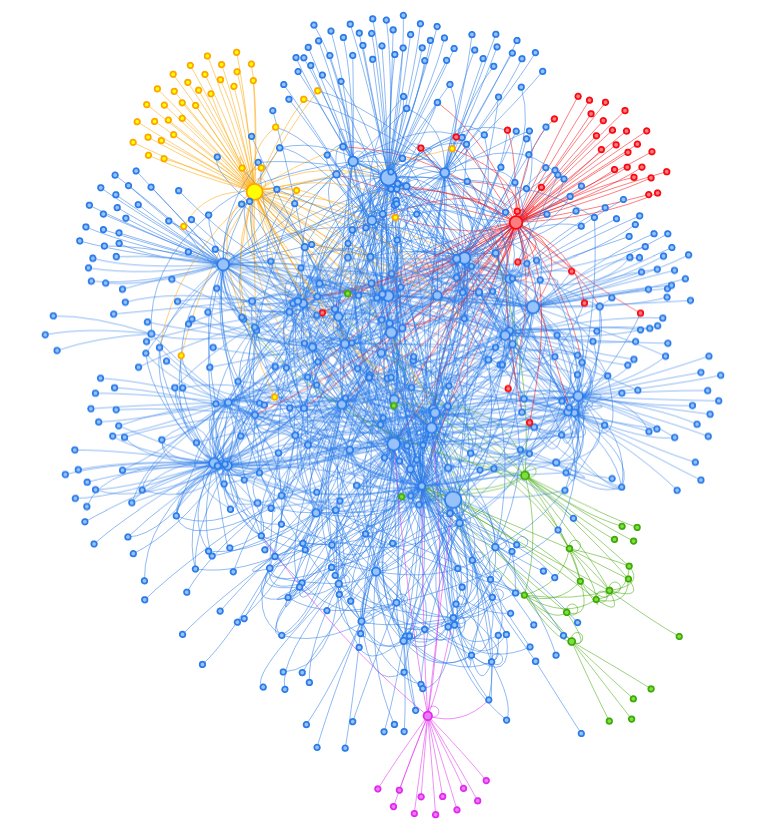
\includegraphics[width=0.35\textwidth]{media/network.png}
    \caption{Dependency Graph\label{fig:dep-graph}}
\end{figure}

As shown in Figure \ref{fig:dep-graph}, these Github projects are very
much interconnected.\\In average, the projects composing our dataset
have 77 dependencies. Among the 77 dependencies, in average, 62
dependencies are shared with at least one other project from our
dataset.

Table \ref{tab:communities} shows the result of the Girvan--Newman
clustering algorithm in terms of centroids and betweenness. The blue
cluster is dominated by Storm from The Apache Software Foundation. Storm
is a distributed real-time computation system. Druid by Alibaba, the
e-commerce company that provides consumer-to-consumer,
business-to-consumer and business-to-business sales services via web
portals, dominates the yellow cluster. In recent years, Alibaba has
become an active member of the open-source community by making some of
its projects publicly available. The red cluster has Hadoop by the
Apache Software Foundation as its centroid. Hadoop is an open-source
software framework for distributed storage and distributed processing of
very large data sets on computer clusters built from commodity hardware.
The green cluster is dominated by the Persistence project of OpenHab.
OpenHab proposes home automation solutions and the Persistence project
is their data access layer. Finally, the purple cluster is dominated by
Libdx by Badlogicgames, which is a cross-platform framework for game
development.

A review of each cluster shows that this partitioning divides projects
in terms of high-level functionalities. For example, the blue cluster is
almost entirely composed of projects from the Apache Software
Foundation. Projects from the Apache Software Foundation tend to build
on top of one another. We also have the red cluster for Hadoop, which is
by itself an ecosystem inside the Apache Software Foundation. Finally,
we obtained a cluster for e-commerce applications (yellow), real-time
network application for home automation (green), and game development
(purple).


\begin{table}[]
\centering
\caption{Communities in terms of ID, Color code, Centroids, Betweenness and number of members}
\label{tab:communities}
\begin{tabular}{llllll}
\#ID               & Community             & Centroids        & Betweenness & \# Members        \\
1                  & Blue                  & Storm &           24525 &    479                                      \\
2                  & Yellow                & Alibaba          & 24400      & 42                                      \\
3                  & Red                   & Hadoop           & 16709      & 37                                      \\
4                  & Green                 & Openhab          & 3504       & 22                                      \\
5                  & Purple                & Libdx              & 6839       & 12                                     
\end{tabular}
\end{table}


\subsection{Building a Database of Defect-Commits and Fix-Commits for
Performances Evaluation}\label{sub:golden}

To build the database against which we assess the performance of BIANCA,
we use the same process as discussed in Section \ref{sec:offline}. We
used Commit-guru to retrieve the complete history of each project and
label commits as defect-commits if they appear to be linked to a closed
issue. The process used by Commit-guru to identify commits that
introduce a defect is simple and reliable in terms of accuracy and
computation time {[}31{]}. We use the commit-guru labels as the baseline
to compute the precision and recall of BIANCA. Each time BIANCA
classifies a commit as \emph{risky}, we can check if the \emph{risky}
commit is in the database of defect-introducing commits. The same
evaluation process is used by related studies {[}13{]}, {[}59--61{]}.
The difference between this \emph{golden} database and the database
described in Section \ref{sec:offline} is that, with this one, we unwind
the whole history instead of building the history as it happens.

\subsection{Process of Comparing New Commits}\label{sec:newcommits}

Because our approach relies on commit pre-hooks to detect risky commit,
we had to find a way to \emph{replay} past commits. To do so, we
\emph{cloned} our test subjects, and then created a new branch called
\emph{BIANCA}. When created, this branch is reinitialized at the initial
state of the project (the first commit) and each commit can be replayed
as they have originally been. For each commit, we store the time taken
for \emph{BIANCA} to run, the number of detected clone pairs, and the
commits that match the current commit. As an example, let's assume that
we have three commits from two projects. At time $t_1$, commit $c_1$ in
project $p_1$ introduces a defect. The defect is experienced by an user
that reports it via an issue $i_1$ at $t_2$. A developer fixes the
defect introduced by $c_1$ in commit $c_2$ and closes $i_1$ at $t_3$.
From $t_3$ we known that $c_1$ introduced a defect using the process
described in Section \ref{sub:golden}. If at $t_4$, $c_3$ is pushed to
$p_2$ and $c_3$ matches $c_1$ after preprocessing, pretty-printing and
formatting, then $c_3$ is classified as \emph{risky} by BIANCA and $c_2$
is proposed to the developer as a potential solution for the defect
introduced in $c_3$.

\begin{figure}

\begin{tikzpicture}
\begin{axis}[
xlabel={Similarity Threshold $\alpha$},
ylabel={Precentage},
legend pos=north west,
xmin=0,
xmax=100
]
\addplot +[mark=none] table [x=alpha, y=f1, col sep=comma] {data/alpha.csv};
\addlegendentry{F$_1$-measure}
\addplot +[mark=none] table [x=alpha, y=precision, col sep=comma] {data/alpha.csv};
\addlegendentry{Precision}
\addplot +[mark=none] table [x=alpha, y=recall, col sep=comma] {data/alpha.csv};
\addlegendentry{Recall}
\addplot +[mark=none] table [x=alpha, y=35, col sep=comma] {data/alpha.csv};
\addlegendentry{$\alpha$ = 35\%}
\end{axis}
\end{tikzpicture}
\caption{Precision, Recall and F$_1$-measure variations according to $\alpha$\label{fig:alpha-deter}}
\end{figure}

To measure the similarity between pairs of commits, we need to decide on
the value of $\alpha$. One possibility would be to test for all possible
values of $\alpha$ and pick the one that provides best accuracy
(F$_1$-measure). The ROC (Receiver Operating Characteristic) curve can
then be used to display the performance of BIANCA with different values
of $\alpha$. Running experiments with all possible $\alpha$ turned out
to be computationally demanding given the large number of commits.
Testing with all the different values of $\alpha$ amounts to $4^{10}$
comparisons.

To address this, we randomly selected a sample of 1\% commits from our
dataset and checked the results by varying $\alpha$ from 1 to 100\%.
Figure \ref{fig:alpha-deter} shows the results. As we can see, there is
a tradeoff between precision and recall, however, after the $\alpha$ =
35\% point, we see a drop in recall; hence, we set $\alpha$ = 35\% in
our experiments. It should also be noted that in clone detection work a
threshold of around 30\% is considered an adequate threshold above which
two code blocks are deemed to be clones, especially for clones of Type
3, which contain added or deleted code statements {[}54{]}, {[}62{]}.
With $\alpha$ = 35\%, the experiments took nearly three months to run on
48 Amazon VPS (Virtual Private Server) running in parallel (4e8
comparisons).

\subsection{Evaluation Measures}\label{evaluation-measures}

Similar to prior work focusing on risky commits (e.g., {[}29{]},
{[}31{]}), we used precision, recall, and F$_1$-measure to evaluate our
approach. They are computed using TP (true positives), FP (false
positives), FN (false negatives), which are defined as follows:

\begin{itemize}
\itemsep1pt\parskip0pt\parsep0pt
\item
  TP: is the number of defect-commits that were properly classified by
  BIANCA
\item
  FP: is the number of healthy commits that were classified by BIANCA as
  risky
\item
  FN: is the number of defect introducing-commits that were not detected
  by BIANCA
\item
  Precision: TP / (TP + FP)
\item
  Recall: TP / (TP + FN)
\item
  F$_1$-measure: 2.(precision.recall)/(precision+recall)
\end{itemize}

It is worth mentioning that, in the case of defect prevention, false
positives can be hard to identify as the defects could be in the code
but not yet reported through a bug report (or issue). To address this,
we did not include the last six months of history. Following similar
studies {[}41{]}, {[}63--65{]}, if a defect is not reported within six
months then it is not considered.

\section{Case Study Results}\label{sec:result}

In this section, we show the effectiveness of BIANCA in detecting risky
commits using clone detection and project dependency analysis. The main
research question addressed by this case study is: Can we detect risky
commits using code comparison within and across related projects, and if
so, what would be the accuracy?

% Please add the following required packages to your document preamble:
% \usepackage{multirow}
% \usepackage{graphicx}
% \usepackage[normalem]{ulem}
% \useunder{\uline}{\ul}{}
\begin{table*}[]
\centering
\caption{BIANCA results in terms of organization, project name, a short description, number of class, number of commits, number of defect introducing commits, number of risky commit detected, precision (\%), recall (\%), F$_1$-measure (\%), the average similarity of first 3 and 5 proposed fixes with the actual fix and the average time difference between detected and original.}
  \label{tab:results}
\resizebox{\textwidth}{!}{%
\begin{tabular}{lllccccccccc}
\hline
Organization                & Project Name                                                  & Short Description                                                        & NoC             & \#Commits        & \begin{tabular}[c]{@{}c@{}}Bug  \\Introducing\\ Commit\end{tabular} & Detected       & Precision      & Recall         & F$_1$          & \begin{tabular}[c]{@{}c@{}}Top 3 \\ Fixes \\Similarity\end{tabular} & \begin{tabular}[c]{@{}c@{}}Top 5\\ Fixes\\ Similarity\end{tabular} \\ \hline
\multirow{4}{*}{Alibaba}    & druid                                                         & Database connection pool                                                 & 3,309           & 4,775            & 1,260                                                            & 787            & 88.44          & 62.46          & 73.21          & 39.97                                                             & 46.69                                                              \\
                            & dubbo                                                         & RPC framework                                                            & 1,715           & 1,836            & 119                                                              & 61             & 96.72          & 51.26          & 67.01          & 60.01                                                             & 57.14                                                              \\
                            & fastjson                                                      & JSON parser/generator                                                    & 2,002           & 1,749            & 516                                                              & 373            & 95.71          & 72.29          & 82.37          & 18.19                                                             & 15.23                                                              \\
                            & jstorm                                                        & Stream Process                                                           & 1,492           & 215              & 24                                                               & 21             & 90.48          & 87.50          & 88.96          & 22.38                                                             & 30.48                                                              \\ \hline
\multirow{2}{*}{Apache}     & hadoop                                                        & Distributed processing                                                   & 9,108           & 14,154           & 3,678                                                            & 851            & 86.84          & 23.14          & 36.54          & 38.94                                                             & 47.68                                                              \\
                            & storm                                                         & Realtime system                                                          & 2,209           & 7,208            & 951                                                              & 444            & 86.26          & 46.69          & 60.58          & 53.03                                                             & 61.10                                                              \\ \hline
Clojure                     & clojure                                                       & Programming language                                                     & 335             & 2,996            & 596                                                              & 46             & 86.96          & 7.72           & 14.18          & 53.61                                                             & 59.52                                                              \\ \hline
\multirow{2}{*}{Dropwizard} & dropwizard                                                    & RESTful web services                                                     & 964             & 3,809            & 581                                                              & 179            & 96.65          & 30.81          & 46.72          & 47.54                                                             & 53.56                                                              \\
                            & metrics                                                       & JVM metrics                                                              & 335             & 1,948            & 331                                                              & 129            & 95.35          & 38.97          & 55.33          & 22.53                                                             & 31.82                                                              \\ \hline
Eclipse                     & che                                                           & Eclipse IDE                                                              & 7,818           & 1,826            & 169                                                              & 9              & 88.89          & 5.33           & 10.05          & 31.01                                                             & 39.04                                                              \\ \hline
Excilys                     & \begin{tabular}[c]{@{}l@{}}Android\\ Annotations\end{tabular} & Android Development                                                      & 1,059           & 2,582            & 566                                                              & 9              & 100.00         & 1.59           & 3.13           & 25.60                                                             & 32.13                                                              \\ \hline
Facebook                    & fresco                                                        & Images Management                                                        & 1,007           & 744              & 100                                                              & 68             & 92.65          & 68.00          & 78.43          & 64.14                                                             & 71.03                                                              \\ \hline
Gocd                        & gocd                                                          & Continuous Delivery server                                               & 16,735          & 3,875            & 499                                                              & 297            & 91.58          & 59.52          & 72.15          & 21.62                                                             & 30.59                                                              \\ \hline
\multirow{4}{*}{Google}     & auto                                                          & source code generators                                                   & 257             & 668              & 124                                                              & 95             & 100.00         & 76.61          & 86.76          & 47.66                                                             & 55.70                                                              \\
                            & guava                                                         & Google Libraries for Java 6+                                             & 1,731           & 3,581            & 973                                                              & 592            & 98.48          & 60.84          & 75.22          & 23.74                                                             & 23.59                                                              \\
                            & guice                                                         & Dependency injection                                                     & 716             & 1,514            & 605                                                              & 104            & 85.58          & 17.19          & 28.63          & 34.77                                                             & 34.53                                                              \\
                            & iosched                                                       & Android App                                                              & 1,088           & 129              & 9                                                                & 6              & 100.00         & 66.67          & 80.00          & 16.50                                                             & 24.97                                                              \\ \hline
Gradle                      & gradle                                                        & Build system                                                             & 11,876          & 37,207           & 6,896                                                            & 1,557          & 97.50          & 22.58          & 36.67          & 23.58                                                             & 19.93                                                              \\ \hline
Jankotek                    & mapdb                                                         & Concurrent datastructures                                                & 267             & 1,913            & 691                                                              & 440            & 94.32          & 63.68          & 76.03          & 63.16                                                             & 72.48                                                              \\ \hline
Jhy                         & jsoup                                                         & Parser                                                                   & 136             & 917              & 254                                                              & 153            & 87.58          & 60.24          & 71.38          & 46.41                                                             & 44.59                                                              \\ \hline
Libdx                       & libgdx                                                        & Java game development                                                    & 4,679           & 12,497           & 3,514                                                            & 1,366          & 87.70          & 38.87          & 53.87          & 57.70                                                             & 56.31                                                              \\ \hline
Netty                       & netty                                                         & Event-driven application                                                 & 2,383           & 7,580            & 3,991                                                            & 1,618          & 89.43          & 40.54          & 55.79          & 63.41                                                             & 62.67                                                              \\ \hline
Openhab                     & openhab                                                       & Home Automation Bus                                                      & 5,817           & 8,826            & 28                                                               & 2              & 100.00         & 7.14           & 13.33          & 28.46                                                             & 30.66                                                              \\ \hline
Openzipkin                  & zipkin                                                        & Distributed tracing system                                               & 397             & 799              & 176                                                              & 73             & 87.67          & 41.48          & 56.31          & 55.92                                                             & 51.90                                                              \\ \hline
Orfjackal                   & retrolambda                                                   & Backport of Java 8's lambda                                              & 171             & 447              & 97                                                               & 35             & 94.29          & 36.08          & 52.19          & 34.69                                                             & 42.06                                                              \\ \hline
OrientTechnologie           & orientdb                                                      & Multi-Model DBMS                                                         & 2,907           & 13,907           & 7,441                                                            & 2,894          & 86.77          & 38.89          & 53.71          & 62.20                                                             & 70.00                                                              \\ \hline
Perwendel                   & spark                                                         & Sinatra  for java                                                        & 205             & 703              & 125                                                              & 82             & 97.56          & 65.60          & 78.45          & 21.88                                                             & 28.00                                                              \\ \hline
PrestoDb                    & presto                                                        & Distributed SQL query                                                    & 4,381           & 8,065            & 2,112                                                            & 991            & 90.62          & 46.92          & 61.83          & 23.34                                                             & 20.64                                                              \\ \hline
RoboGuice                   & roboguice                                                     & Google Guice on Android                                                  & 1,193           & 1,053            & 229                                                              & 70             & 91.43          & 30.57          & 45.82          & 53.81                                                             & 56.55                                                              \\ \hline
Lombok                      & lombok                                                        & \begin{tabular}[c]{@{}l@{}}Additions to the\\ Java language\end{tabular} & 1,146           & 1,872            & 560                                                              & 212            & 91.98          & 37.86          & 53.64          & 58.94                                                             & 57.49                                                              \\ \hline
Scribejava                  & scribejava                                                    & OAuth library                                                            & 218             & 609              & 72                                                               & 16             & 93.75          & 22.22          & 35.93          & 30.05                                                             & 38.16                                                              \\ \hline
\multirow{6}{*}{Square}     & dagger                                                        & Dependency injector                                                      & 232             & 697              & 144                                                              & 84             & 90.48          & 58.33          & 70.93          & 64.29                                                             & 64.97                                                              \\
                            & javapoet                                                      & Java API                                                                 & 66              & 650              & 163                                                              & 113            & 100.00         & 69.33          & 81.88          & 51.04                                                             & 53.20                                                              \\
                            & okhttp                                                        & HTTP+HTTP/2 client                                                       & 344             & 2,649            & 592                                                              & 474            & 93.04          & 80.07          & 86.07          & 29.09                                                             & 24.91                                                              \\
                            & okio                                                          & I/O API for Java                                                         & 90              & 433              & 40                                                               & 24             & 100.00         & 60.00          & 75.00          & 31.51                                                             & 35.50                                                              \\
                            & otto                                                          & Guava-based event bus                                                    & 84              & 201              & 15                                                               & 15             & 93.33          & 100.00         & 96.55          & 54.11                                                             & 49.94                                                              \\
                            & retrofit                                                      & Type-safe HTTP client                                                    & 202             & 1,349            & 151                                                              & 111            & 99.10          & 73.51          & 84.41          & 49.88                                                             & 45.46                                                              \\ \hline
StephaneNicolas             & robospice                                                     & Android library                                                          & 461             & 865              & 113                                                              & 39             & 87.18          & 34.51          & 49.45          & 60.90                                                             & 65.04                                                              \\ \hline
ThinkAurelius               & titan                                                         & Graph Database                                                           & 2,015           & 4,434             & 1,634                                                            & 527            & 90.13          & 32.25          & 47.51          & 48.64                                                             & 50.59                                                              \\ \hline
Jedis                       & jedis                                                         & Redis client                                                             & 203             & 1,370             & 295                                                              & 226            & 92.04          & 76.61          & 83.62          & 25.69                                                             & 29.45                                                              \\ \hline
Yahoo                       & anthelion                                                     & Plugin for Apache Nutch                                                  & 1,620            & 7                & 0                                                                & -              & -              & -              & -              & -                                                                 & -                                                                  \\ \hline
Zxing                       & zxing                                                         & 1D/2D barcode image                                                      & 3,030           & 3,253            & 791                                                              & 123            & 94.31          & 15.55          & 26.70          & 29.35                                                             & 37.96                                                              \\ \hline
\textbf{Total}              & \textbf{}                                                     & \textbf{}                                                                & \textbf{96,003} & \textbf{165,912} & \textbf{41,225}                                                  & \textbf{15316} & \textbf{90.75} & \textbf{37.15} & \textbf{52.72} & \textbf{40.78}                                                    & \textbf{44.17}                                                     \\ \hline
\end{tabular}%
}
\end{table*}

Table \ref{tab:results} shows the results of applying BIANCA in terms of
the organization, project name, a short description of the project, the
number of classes, the number of commits, the number of defect-commits,
the number of defect-commits detected by BIANCA, precision (\%), recall
(\%), F$_1$-measure and the average difference, in days, between
detected commit and the \emph{original} commit inserting the defect for
the first time.

With $\alpha$ = 35\%, BIANCA achieves, on average, a precision of
90.75\% (13,899/15,316) commits identified as risky. These commits
triggered the opening of an issue and had to be fixed later on. On the
other hand, BIANCA achieves, on average, 37.15\% recall (15,316/41,225),
and an average F$_1$ measure of 52.72\%. The relatively \emph{low}
recall is to be expected, since BIANCA considers risky commits that are
also in other projects.

Also, out of the 15,316 commits BIANCA classified as \emph{risky}, only
1,320 (8.6\%) were because they were matching a defect-commit inside the
same project. This finding supports the idea that developers of a
project are not likely to introduce the same defect twice while
developers of different projects that share dependencies are, in fact,
likely to introduce similar defects. We believe this is an important
finding for researchers aiming to achieve cross-project defect
prevention, regardless of the technique (e.g., statistical model, AST
comparison, code comparison, etc.) employed.

It is important to note that we do not claim that 37.15\% of issues in
open-source systems are caused by project dependencies. To support such
a claim, we would need to analyse the 15,316 detected defect-commits and
determine how many yield defects that are similar across projects.
Studying the similarity of defects across projects is a complex task and
may require analysing the defect reports manually. This is left as
future work. This said, we showed, in this paper, that software systems
sharing dependencies also share common issues, irrespective to whether
these issues represent similar defects or not.

In the following subsections, we compare BIANCA with a random
classifier, assess the quality of the proposed fixes, and present the
findings of our manual analysis.

\subsection{Random Classifier
Comparison}\label{random-classifier-comparison}

Although our average F$_1$ measure of 52.72\% may seem low at first
glance, achieveing a high F$_1$ measure for unbalanced data is very
difficult {[}66{]}. Therefore, a common appraoch to ground detection
results is to compare it to a simple baseline.

The random classifier first generates a random number $n$ between 0 and
1 for the 165,912 commits composing our dataset. For each commit, if $n$
is greater than 0.5, then the commit is classified as risky and vice
versa. As expected by a random classifier, our implementation detected
\textasciitilde{}50\% (82,384 commits) of the commits to be
\emph{risky}. It is worth mentioning is that the random classifier
achieved 24.9\% precision, 49.96\% recall and 33.24\% F$_1$-measure.
Since our data is unbalanced (i.e., there are many more \emph{healthy}
than \emph{risky} commits) these numbers are to be expected for a random
classifier. Indeed, the recall is very close to 50\% since a commit can
take on one of two classifications, risky or non-risky. While analysing
the precision, however, we can see that the data is unbalanced (a random
classifier would achieve a precision of 50\% on a balanced dataset).

It is important to note that the purpose of this analysis is not to say
that we outperform a simple random classifier, rather to shed light on
the fact that our dataset is unbalanced and achieving an average F$_1$ =
52.72\% is non-trivial, especially when a baseline only achieves an
F$_1$-measure of 33.24\%.

\subsection{Analysis of the Quality of the Fixes Proposed by
BIANCA}\label{analysis-of-the-quality-of-the-fixes-proposed-by-bianca}

One of the advantages of BIANCA over other techniques is that it also
proposes fixes for the \emph{risky} commits it detects. In order to
evaluate the quality of the proposed fixes, we compare the proposed
fixes with the actual fixes provided by the developers. To do so, we
used the same preprocessing steps we applied to incoming commits:
extract, pretty-print, normalize and filter the blocks modified by the
proposed and actual fixes. Then, the blocks of the actual fixes and the
proposed fixes can be compared with our clone comparison engine.

Similar to other studies recommending fixes, we assess the quality of
the first 3 and 5 proposed fixes {[}32--37{]}. The average similarity of
the first 3 fixes is 40.78\% while the similarity of the first five
fixes is 44.17\%. Results are reported in Table \ref{tab:results}.

In the framework of this study, for a fix to be ranked as qualitative it
has to reach our $\alpha$=35\% similarity threshold. Meaning that the
proposed fixed must be at least 35\% similar to the actual fix. On
average, the proposed fixes are above the $\alpha$=35\% threshold. On a
per commit basis, BIANCA proposed 101,462 fixes for the 13,899 true
positives \emph{risky commits} (7.3 per commit). Out of the 101,462
proposed fixes, 78.67\% are above our $\alpha$=35\% threshold.

In other words, BIANCA is able to detect \emph{risky} commits with
90.75\% precision, 37.15\% recall, and proposes fixes that contain, on
average, 40-44\% of the actual code needed to transform the \emph{risky}
commit into a \emph{non-risky} one. It is still too early to claim
whether BIANCA's recommendations can be useful to developers. For this,
we need to conduct user study, which we plan to do as future work.

\subsection{Manual Analysis}\label{manual-analysis}

BIANCA performed best when applied to three projects: Otto by Square
(100.00\% precision and 76.61\% recall, 96.55\% F$_1$-measure), JStorm
by Alibaba (90.48\% precision, 87.50\% recall, 88.96\% F$_1$-measure),
and Auto by Google (90.48\% precision, 87.50\% recall, 86.76\%
F$_1$-measure). It performed worst when applied to Android Annotations
by Excilys (100.00\% precision, 1.59\% recall, 3.13\% F$_1$-measure) and
Che by Eclipse (88.89\% precision, 5.33\% recall, 10.05\%
F$_1$-measure), Openhab by Openhab (100.00\% precision, 7.14\% recall,
13.33\% F$_1$-measure). To understand the performance of BIANCA, we
conducted a manual analysis of the commits classified as \emph{risky} by
BIANCA for these projects.

\subsubsection{Otto by Square (F$_1$-measure =
96.5\%)}\label{otto-by-square-fux5f1-measure-96.5}

At first, the F$_1$-measure of Otto by Square seems surprising given the
specific set of features it provides. Otto provides a Guava-based event
bus. While it does have dependencies that makes it vulnerable to defects
in related projects, the fact that it provides specific features makes
it, at first sight, unlikely to share defects with other projects.
Through our manual analysis, we found that out of the 16 \emph{risky}
commits detected by BIANCA, only 11 (68.75\%) matched defect-introducing
commits inside the Otto project itself. This is significantly higher
than the average number of single-project defects (8.6\%). Further
investigation of the project management system revealed that a very few
issues have been submitted for this project (15) and, out of the 11
matches inside the Otto project, 7 were aiming to fix the same issue
that had been submitted and fixed several times instead of re-opening
the original issue.

\subsubsection{JStorm by Alibaba (F$_1$-measure =
88.96\%)}\label{jstorm-by-alibaba-fux5f1-measure-88.96}

For JStorm by Alibaba, our manual analysis of the \emph{risky} commits
revealed that, in addition to providing stream processes, JStorm mainly
supports JSON. The commits detected as \emph{risky} were related to the
JSON encoding/decoding functionalities of JStorm. In our dataset, we
have several other projects that supports JSON encoding and decoding
such as FastJSON by Alibaba, Hadoop by Apache, Dropwizard by Dropwizard,
Gradle by Gradle and Anthelion by Yahoo. There is, however, only one
project supporting JSON in the same cluster as JStorm, Fastjson by
Alibaba. FastJSON has a rather large history of defect-commits (516) and
18 out of the 21 commits marked as \emph{risky} by BIANCA were marked so
because they matched defect-commits in the FastJSON project.

\subsubsection{Auto by Google (F$_1$-measure =
86.76\%)}\label{auto-by-google-fux5f1-measure-86.76}

Google Auto is a code generation engine. This code generation engine is
used by other Google projects in our database, such as Guava and Guice.
Most of the Google Auto \emph{risky} commits (79\%) matched commits in
the Guava and the Guice project. As Guice and Guave share the same
code-generation engine (Auto), it makes sense that code introducing
defects in these projects share the characteristics of commits
introducing defects in Auto.

\subsubsection{Openhab by Openhab (F$_1$-measure =
13.33\%)}\label{openhab-by-openhab-fux5f1-measure-13.33}

Openhab by Openhab provides bus for home automation or smart homes. This
is a very specific set of feature. Moreover, Openhab and its
dependencies are alone in the green cluster. In other words, the only
project against which BIANCA could have checked for matching defects is
Openhab itself. BIANCA was able to detect 2/28 bugs for Openhab. We
believe that if we had other home-automation projects in our dataset
(such as \emph{HomeAutomation} a component based for smart home systems
{[}67{]}) then we would have achieved a better F$_1$-measure.

\subsubsection{Che by Eclipse (F$_1$-measure =
10.05\%)}\label{che-by-eclipse-fux5f1-measure-10.05}

Eclipse Che is part of the Eclipse IDE ttha provides development support
for a wide range of programming languages such as C, C++, Java and
others. Despite the fact that the Che project has a decent amount of
defect-commits (169) and that it is in the blue cluster (dominated by
Apache,) BIANCA was only able to detect 9 \emph{risky} commits. After
manual analysis of the 169 defect-commits, we were not able to draw any
conclusion on why we were not able to achieve better performance. We can
only assume that Eclipse's developers are particularly careful about how
they use their dependencies and the quality of their code in general.
Only 2\% (169/7,818) of their commits introduce new defects.

\subsubsection{Annotations by Excilys (F$_1$-measure =
3.13\%)}\label{annotations-by-excilys-fux5f1-measure-3.13}

The last project we analysed manually is Annotations by Excilys. Very
much like Openhab by Openhab, it provides a very particular set of
features, which consist of Java annotations for Android projects. We do
not have any other project related to Java annotations or the Android
ecosystem at large. This caused BIANCA to perform poorly.

Our interpretation of the manual analysis of the best and worst
performing projects is that BIANCA performs best when applied to
clusters that contain projects that are similar in terms of features,
domain or intent. These projects tend to be interconnected through
dependencies. In the future, we intend to study the correlation between
the cluster betweenness measure and the performance of BIANCA.

\section{Threats to Validity}\label{sec:threats}

The selection of target systems is one of the common threats to validity
for approaches aiming to improve the analysis of software systems. It is
possible that the selected programs share common properties that we are
not aware of and therefore, invalidate our results. However, the systems
analysed by BIANCA were selected from Github based on their popularity
and the ability to mine their past issues and also to retrieve their
dependencies. Any project that satisfies these criteria would be
included in the analysis. Moreover, the systems vary in terms of
purpose, size, and history. In addition, we see a threat to validity
that stems from the fact that we only used open-source systems. The
results may not be generalizable to industrial systems. We intend to
undertake these studies in future work.

The programs we used in this study are all based on the Java programming
language. This can limit the generalization of the results to pojects
written in other languages. However, similar to Java, one can write a
TXL grammar for a new language then BIANCA can work since BIANCA relies
on TXL. Finally, we use NICAD as the code comparison engine. The
accuracy of NICAD affects the accuracy of BIANCA. This said, since NICAD
has been tested on large systems, we are confident that it is a suitable
engine for comparing code using TXL. Also, there is nothing that
prevents us from using other text-based code comparisons engines, if
need be. In conclusion, internal and external validity have both been
minimized by choosing a set of 42 different systems, using input data
that can be found in any programming languages and version systems
(commit and changesets).

\section{Conclusion}\label{sec:conclusion}

In this paper, we presented BIANCA (Bug Insertion ANticipation by Clone
Analysis at commit time), an approach that detects risky commits (i.e.,
a commit that is likely to introduce a bug) with 90.75\% precision and
37.15\% recall. BIANCA uses clone detection techniques and project
dependency analysis to detect risky commits within and across dependant
projects. BIANCA operates at commit-time, i.e., before the commits reach
the central repository. In addition, because it relies on code
comparison, BIANCA does not only detect risky commits but also makes
recommendations to developers on how to fix them. We believe that this
makes BIANCA a practical approach for preventing bugs and proposing
corrective measures that integrates well with the developers work flow
through the commit mechanism.

To build on this work, we need to conduct a human study with developers
in order to gather their feedback on the approach. The feedback obtained
will help us fine-tune the approach. Also, we want to examine the
relationship between project cluster measures (such as betweenness) and
the performance of BIANCA. Finally, another improvement to BIANCA would
be to support Type 4 clones.

\newpage

\section{References}\label{references}

\small

{[}1{]} D. Lo, ``A Comparative Study of Supervised Learning Algorithms
for Re-opened Bug Prediction,'' in \emph{2013 17th european conference
on software maintenance and reengineering}, 2013, pp. 331--334.

{[}2{]} J. Nam, S. J. Pan, and S. Kim, ``Transfer defect learning,'' in
\emph{2013 35th international conference on software engineering
(iCSE)}, 2013, pp. 382--391.

{[}3{]} C. Lewis, Z. Lin, C. Sadowski, X. Zhu, R. Ou, and E. J.
{Whitehead Jr.}, ``Does bug prediction support human developers?
findings from a google case study,'' in \emph{International conference
on software engineering (iCSE) (2013)}, 2013, pp. 372--381.

{[}4{]} B. Johnson, Y. Song, E. Murphy-Hill, and R. Bowdidge, ``Why
don't software developers use static analysis tools to find bugs?'' in
\emph{35th international conference on software engineering (iCSE)},
2013, pp. 672--681.

{[}5{]} The Apache Software Foundation, ``Apache BatchEE.'' 2015.

{[}6{]} Graphwalker, ``GraphWalker for testers.'' 2016.

{[}7{]} {Joshua O'Madadhain, Danyel Fisher, Scott White, Padhraic
Smyth}Y.-b. B., ``Analysis and Visualization of Network Data using
JUNG,'' \emph{Journal of Statistical Software}, vol. 10, no. 2, pp.
1--35, 2005.

{[}8{]} Chris Vignola, ``The Java Community Process(SM) Program - JSRs:
Java Specification Requests - detail JSR\# 352.'' 2014.

{[}9{]} S. Chidamber and C. Kemerer, ``A metrics suite for object
oriented design,'' \emph{IEEE Transactions on Software Engineering},
vol. 20, no. 6, pp. 476--493, Jun. 1994.

{[}10{]} N. Moha, F. Palma, M. Nayrolles, and B. J. Conseil,
``Specification and Detection of SOA Antipatterns,'' in
\emph{International conference on service oriented computing}, 2012, pp.
1--16.

{[}11{]} L. Briand, J. Daly, and J. Wust, ``A unified framework for
coupling measurement in object-oriented systems,'' \emph{IEEE
Transactions on Software Engineering}, vol. 25, no. 1, pp. 91--121,
1999.

{[}12{]} V. Basili, L. Briand, and W. Melo, ``A validation of
object-oriented design metrics as quality indicators,'' \emph{IEEE
Transactions on Software Engineering}, vol. 22, no. 10, pp. 751--761,
1996.

{[}13{]} K. {El Emam}, W. Melo, and J. C. Machado, ``The prediction of
faulty classes using object-oriented design metrics,'' \emph{Journal of
Systems and Software}, vol. 56, no. 1, pp. 63--75, Feb. 2001.

{[}14{]} R. Subramanyam and M. Krishnan, ``Empirical analysis of CK
metrics for object-oriented design complexity: implications for software
defects,'' \emph{IEEE Transactions on Software Engineering}, vol. 29,
no. 4, pp. 297--310, Apr. 2003.

{[}15{]} T. Gyimothy, R. Ferenc, and I. Siket, ``Empirical validation of
object-oriented metrics on open source software for fault prediction,''
\emph{IEEE Transactions on Software Engineering}, vol. 31, no. 10, pp.
897--910, Oct. 2005.

{[}16{]} M. Nayrolles, A. Maiga, A. Hamou-lhadj, and A. Larsson, ``A
Taxonomy of Bugs : An Empircial Study,'' pp. 1--10.

{[}17{]} M. Nayrolles, ``Improving SOA Antipattern Detection in Service
Based Systems by Mining Execution Traces,'' PhD thesis, 2013.

{[}18{]} A. Demange, N. Moha, and G. Tremblay, ``Detection of SOA
Patterns,'' in \emph{International conference on service-oriented
computing}, 2013, pp. 114--130.

{[}19{]} F. Palma, ``Detection of SOA Antipatterns,'' PhD thesis, Ecole
Polytechnique de Montreal, 2013.

{[}20{]} N. Nagappan and T. Ball, ``Static analysis tools as early
indicators of pre-release defect density,'' in \emph{Proceedings of the
27th international conference on software engineering - iCSE '05}, 2005,
p. 580.

{[}21{]} N. Nagappan, T. Ball, and A. Zeller, ``Mining metrics to
predict component failures,'' in \emph{Proceeding of the 28th
international conference on software engineering - iCSE '06}, 2006, p.
452.

{[}22{]} T. Zimmermann, R. Premraj, and A. Zeller, ``Predicting Defects
for Eclipse,'' in \emph{Third international workshop on predictor models
in software engineering (pROMISE'07: iCSE workshops 2007)}, 2007, pp.
9--9.

{[}23{]} T. Zimmermann and N. Nagappan, ``Predicting defects using
network analysis on dependency graphs,'' in \emph{Proceedings of the
13th international conference on software engineering - iCSE '08}, 2008,
p. 531.

{[}24{]} N. Nagappan and T. Ball, ``Use of relative code churn measures
to predict system defect density,'' in \emph{Proceedings. 27th
international conference on software engineering, 2005.}, 2005, pp.
284--292.

{[}25{]} A. Hassan and R. Holt, ``The top ten list: dynamic fault
prediction,'' in \emph{21st iEEE international conference on software
maintenance (iCSM'05)}, 2005, pp. 263--272.

{[}26{]} T. Ostrand, E. Weyuker, and R. Bell, ``Predicting the location
and number of faults in large software systems,'' \emph{IEEE
Transactions on Software Engineering}, vol. 31, no. 4, pp. 340--355,
Apr. 2005.

{[}27{]} S. Kim, T. Zimmermann, E. J. {Whitehead Jr.}, and A. Zeller,
``Predicting Faults from Cached History,'' in \emph{29th international
conference on software engineering (iCSE'07)}, 2007, pp. 489--498.

{[}28{]} F. Rahman and P. Devanbu, ``How, and why, process metrics are
better,'' in \emph{Proceedings of the 2013 international conference on
software engineering}, 2013, pp. 432--441.

{[}29{]} S. {Sunghun Kim}, E. Whitehead, and Y. {Yi Zhang},
``Classifying Software Changes: Clean or Buggy?'' \emph{IEEE
Transactions on Software Engineering}, vol. 34, no. 2, pp. 181--196,
Mar. 2008.

{[}30{]} A. E. Hassan, ``Predicting faults using the complexity of code
changes,'' in \emph{2009 iEEE 31st international conference on software
engineering}, 2009, pp. 78--88.

{[}31{]} Y. Kamei, E. Shihab, B. Adams, A. E. Hassan, A. Mockus, A.
Sinha, and N. Ubayashi, ``A large-scale empirical study of just-in-time
quality assurance,'' \emph{IEEE Transactions on Software Engineering},
vol. 39, no. 6, pp. 757--773, Jun. 2013.

{[}32{]} K. Pan, S. Kim, and E. J. Whitehead, ``Toward an understanding
of bug fix patterns,'' \emph{Empirical Software Engineering}, vol. 14,
no. 3, pp. 286--315, Aug. 2008.

{[}33{]} D. Kim, J. Nam, J. Song, and S. Kim, ``Automatic patch
generation learned from human-written patches,'' in \emph{2013 35th
international conference on software engineering (iCSE)}, 2013, vol. 1,
pp. 802--811.

{[}34{]} Y. Tao, J. Kim, S. Kim, and C. Xu, ``Automatically generated
patches as debugging aids: a human study,'' in \emph{Proceedings of the
22nd aCM sIGSOFT international symposium on foundations of software
engineering}, 2014, pp. 64--74.

{[}35{]} V. Dallmeier, A. Zeller, and B. Meyer, ``Generating Fixes from
Object Behavior Anomalies,'' in \emph{24th iEEE/aCM international
conference on automated software engineering}, 2009, pp. 550--554.

{[}36{]} C. {Le Goues}, M. Dewey-Vogt, S. Forrest, and W. Weimer, ``A
systematic study of automated program repair: Fixing 55 out of 105 bugs
for \$8 each,'' in \emph{2012 34th international conference on software
engineering (iCSE)}, 2012, pp. 3--13.

{[}37{]} X.-B. D. Le, T.-D. B. Le, and D. Lo, ``Should fixing these
failures be delegated to automated program repair?'' in \emph{Software
reliability engineering (iSSRE), 2015 iEEE 26th international symposium
on}, 2015, pp. 427--437.

{[}38{]} M. Girvan and M. E. J. Newman, ``Community structure in social
and biological networks,'' \emph{Proceedings of the National Academy of
Sciences}, vol. 99, no. 12, pp. 7821--7826, Jun. 2002.

{[}39{]} M. E. J. Newman and M. Girvan, ``Finding and evaluating
community structure in networks,'' \emph{Physical Review E}, vol. 69,
no. 2, p. 026113, Feb. 2004.

{[}40{]} R. Wu, H. Zhang, S. Kim, and S. Cheung, ``Relink: recovering
links between bugs and changes,'' in \emph{Proceedings of the 19th aCM
sIGSOFT symposium and the 13th european conference on foundations of
software engineering.}, 2011, pp. 15--25.

{[}41{]} C. Rosen, B. Grawi, and E. Shihab, ``Commit guru: analytics and
risk prediction of software commits,'' in \emph{Proceedings of the 2015
10th joint meeting on foundations of software engineering - eSEC/fSE
2015}, 2015, pp. 966--969.

{[}42{]} A. Hindle, D. M. German, and R. Holt, ``What do large commits
tell us?'' in \emph{Proceedings of the 2008 international workshop on
mining software repositories - mSR '08}, 2008, p. 99.

{[}43{]} S. Kim, T. Zimmermann, K. Pan, and E. {Jr. Whitehead},
``Automatic Identification of Bug-Introducing Changes,'' in \emph{21st
iEEE/aCM international conference on automated software engineering
(aSE'06)}, 2006, pp. 81--90.

{[}44{]} Y. Kamei, E. Shihab, B. Adams, A. E. Hassan, A. Mockus, A.
Sinha, and N. Ubayashi, ``A large-scale empirical study of just-in-time
quality assurance,'' \emph{IEEE Transactions on Software Engineering},
vol. 39, no. 6, pp. 757--773, Jun. 2013.

{[}45{]} J. R. Cordy, ``Source transformation, analysis and generation
in TXL,'' in \emph{Proceedings of the 2006 aCM sIGPLAN symposium on
partial evaluation and semantics-based program manipulation - pEPM '06},
2006, p. 1.

{[}46{]} T. R. Dean, J. R. Cordy, A. J. Malton, and K. A. Schneider,
``Agile Parsing in TXL,'' in \emph{Proceedings of iEEE international
conference on automated software engineering}, vol. 10, pp. 311--336.

{[}47{]} B. Bultena and F. Ruskey, ``An Eades-McKay algorithm for
well-formed parentheses strings,'' \emph{Information Processing
Letters}, vol. 68, no. 5, pp. 255--259, 1998.

{[}48{]} J. H. Johnson, ``Identifying redundancy in source code using
fingerprints,'' in \emph{CASCON '93 proceedings of the 1993 conference
of the centre for advanced studies on collaborative research: software
engineering - volume 1}, 1993, pp. 171--183.

{[}49{]} J. H. Johnson, ``Visualizing textual redundancy in legacy
source,'' in \emph{Proceedings of the 1994 conference of the centre for
advanced studies on collaborative research}, 1994, p. 32.

{[}50{]} A. Marcus and J. Maletic, ``Identification of high-level
concept clones in source code,'' in \emph{Proceedings 16th annual
international conference on automated software engineering (aSE 2001)},
pp. 107--114.

{[}51{]} U. Manber, ``Finding similar files in a large file system,'' in
\emph{Usenix winter}, 1994, pp. 1--10.

{[}52{]} S. Ducasse, M. Rieger, and S. Demeyer, ``A Language Independent
Approach for Detecting Duplicated Code.''

{[}53{]} R. Wettel and R. Marinescu, ``Archeology of code duplication:
recovering duplication chains from small duplication fragments,'' in
\emph{Seventh international symposium on symbolic and numeric algorithms
for scientific computing (sYNASC'05)}, 2005, p. 8 pp.

{[}54{]} J. R. Cordy and C. K. Roy, ``The NiCad Clone Detector,'' in
\emph{2011 iEEE 19th international conference on program comprehension},
2011, pp. 219--220.

{[}55{]} C. Kapser and M. W. Godfrey, ``Toward a Taxonomy of Clones in
Source Code: A Case Study,'' in \emph{International workshop on
evolution of large scale industrial software architectures}, 2003, pp.
67--78.

{[}56{]} CHANCHAL K. ROY, ``Detection and Analysis of Near-Miss Software
Clones,'' PhD thesis, Queen's University, 2009.

{[}57{]} S. Ducasse, M. Rieger, and S. Demeyer, ``A language independent
approach for detecting duplicated code,'' in \emph{Proceedings iEEE
international conference on software maintenance - 1999 (iCSM'99).
'software maintenance for business change' (cat. no.99CB36360)}, 1999,
pp. 109--118.

{[}58{]} J. W. Hunt and T. G. Szymanski, ``A fast algorithm for
computing longest common subsequences,'' \emph{Communications of the
ACM}, vol. 20, no. 5, pp. 350--353, May 1977.

{[}59{]} T. Lee, J. Nam, D. Han, S. Kim, and H. P. In, ``Micro
interaction metrics for defect prediction,'' in \emph{Proceedings of the
19th aCM sIGSOFT symposium and the 13th european conference on
foundations of software engineering - sIGSOFT/fSE '11}, 2011, p. 311.

{[}60{]} P. Bhattacharya and I. Neamtiu, ``Bug-fix time prediction
models: can we do better?'' in \emph{Proceeding of the 8th working
conference on mining software repositories - mSR '11}, 2011, p. 207.

{[}61{]} S. Kpodjedo, F. Ricca, P. Galinier, Y.-G. Gu{é}h{é}neuc, and G.
Antoniol, ``Design evolution metrics for defect prediction in object
oriented systems,'' \emph{Empirical Software Engineering}, vol. 16, no.
1, pp. 141--175, Dec. 2010.

{[}62{]} C. K. Roy and J. R. Cordy, ``An Empirical Study of Function
Clones in Open Source Software,'' in \emph{2008 15th working conference
on reverse engineering}, 2008, pp. 81--90.

{[}63{]} C. Rosen, B. Grawi, and E. Shihab, ``Commit guru: analytics and
risk prediction of software commits,'' in \emph{Proceedings of the 2015
10th joint meeting on foundations of software engineering - eSEC/fSE
2015}, 2015, pp. 966--969.

{[}64{]} T.-h. Chen, M. Nagappan, E. Shihab, and A. E. Hassan, ``An
Empirical Study of Dormant Bugs Categories and Subject Descriptors,'' in
\emph{Mining software repository}, 2014, pp. 82--91.

{[}65{]} E. Shihab, A. Ihara, Y. Kamei, W. M. Ibrahim, M. Ohira, B.
Adams, A. E. Hassan, and K. I. Matsumoto, ``Studying re-opened bugs in
open source software,'' \emph{Empirical Software Engineering}, vol. 18,
no. 5, pp. 1005--1042, 2013.

{[}66{]} T. Menzies, A. Dekhtyar, J. Distefano, and J. Greenwald,
``Problems with Precision: A Response to` Comments on'Data Mining Static
Code Attributes to Learn Defect Predictors'','' \emph{IEEE Transactions
on Software Engineering}, vol. 33, no. 9, p. 637, 2007.

{[}67{]} L. Seinturier, P. Merle, R. Rouvoy, D. Romero, V. Schiavoni,
and J.-b. Stefani, ``A Component-Based Middleware Platform for
Reconfigurable Service-Oriented Architectures,'' \emph{Software-Practice
and experience}, vol. 5, pp. 1--26, 2012.



\end{document}
